\documentclass[12pt,a4paper,oneside]{book}

\usepackage[utf8]{inputenc}
\usepackage[T1]{fontenc}
\usepackage[backend=biber,style=numeric,sorting=none]{biblatex}
\usepackage[margin=2.5cm]{geometry}
\usepackage[hidelinks]{hyperref}
\usepackage{amsmath}
\usepackage{amssymb}
\usepackage{graphicx}

\addbibresource{references.bib}

\title{%
    \vspace{2cm}%
    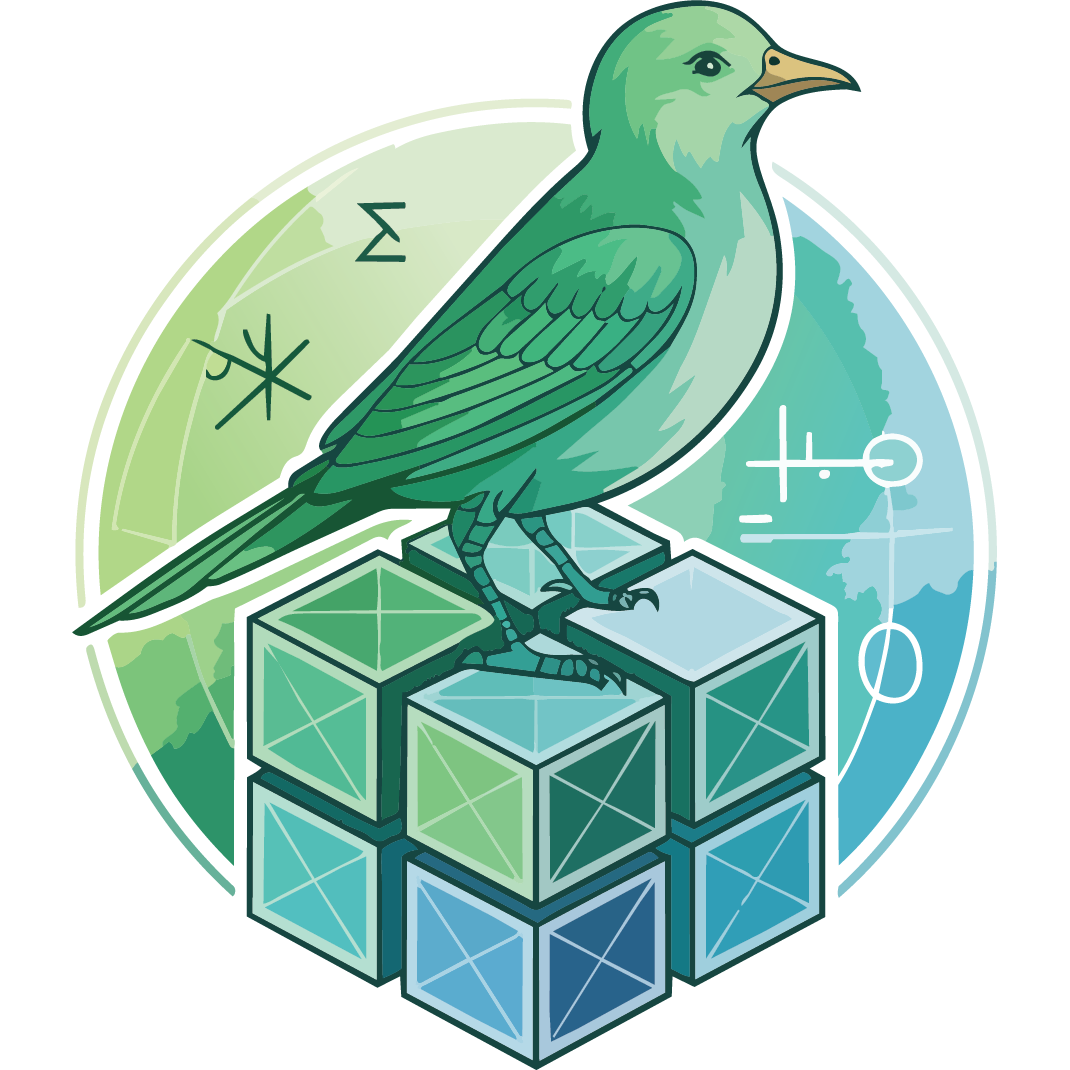
\includegraphics[width=4cm]{../_shared/logo/logo.png}\\[1cm]%
    Thesis Title
}
\author{The Author}
\date{}

\begin{document}

\frontmatter
\maketitle

\chapter*{Abstract}
\addcontentsline{toc}{chapter}{Abstract}

This is a minimal example of the kind of multi-chapter thesis-style
document \texttt{rules\_latex} can build hermetically. It demonstrates
biblatex for citations, the \texttt{book} class for chapter
structure, and the use of \texttt{\textbackslash input} to break
the document up into chapter files.

\tableofcontents

\mainmatter

\chapter{Introduction}
\label{ch:introduction}

The introduction motivates the work. It typically:

\begin{itemize}
    \item States the problem.
    \item Argues that the problem is important.
    \item Outlines the contributions of the thesis.
    \item Foreshadows the chapter structure that follows.
\end{itemize}

In this minimal example the problem is: \emph{how do we produce
hermetic, reproducible builds of LaTeX documents?} The contributions
are: a Bazel rule set built around Tectonic; an implicit cache
pipeline that hides the complexity of package management from
users; and a live-preview workflow that matches Overleaf's
ergonomics. Subsequent chapters expand each contribution.

\chapter{Background}
\label{ch:background}

Bazel is a content-addressed build system originally developed inside
Google~\cite{google2007blaze}. Tectonic is a self-contained TeX/LaTeX
engine derived from XeTeX~\cite{tectonic2025}. The combination has
appealing properties for reproducible document
production~\cite{morgenthaler2012searching}.

Both projects emphasise hermeticity, but neither solves the problem
end-to-end on its own. Bazel needs an actual TeX engine to invoke;
Tectonic needs an external manager to handle multi-document builds,
caching, and cross-project sharing. \texttt{rules\_latex} fills the
gap.

\chapter{Results}
\label{ch:results}

A real thesis would have results here. This placeholder chapter
exists to show how a multi-chapter \texttt{book}-class document
strings together via \texttt{\textbackslash input}.

When this example is built, Bazel invokes Tectonic once to produce
the PDF and biber once to resolve the bibliography. Both runs are
sandboxed; their inputs are the union of \texttt{main.tex}, every
\texttt{chapters/*.tex} file, and \texttt{references.bib}.


\backmatter
\printbibliography[heading=bibintoc]

\end{document}
